\documentclass[tikz,border=10pt]{standalone}
\begin{document}
% repair: all stroke widths set to 1.2pt (middle weight), round joins
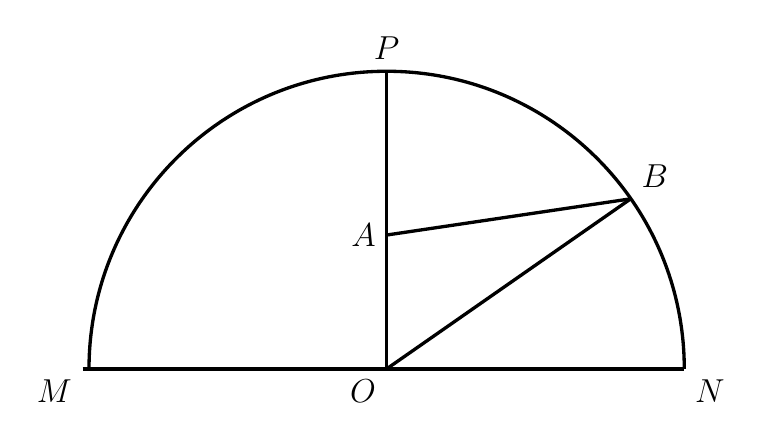
\begin{tikzpicture}[line join=round, line width=1.2pt]
% named coordinates (scale s = 0.016064 cm/px, y flipped, origin at O)
\coordinate (L) at (-3.86,0);     % left diameter end (labelled M)
\coordinate (O) at (0,0);         % centre
\coordinate (N) at (3.78,0);      % right diameter end
\coordinate (P) at (0,3.79);      % top of semicircle
\coordinate (A) at (0,1.70);      % on segment OP
\coordinate (B) at (3.10,2.16);   % on arc

% diameter and upper semicircle, 1.2pt
\draw[line width=1.2pt] (L) -- (N);
\draw[line width=1.2pt] (N) arc[start angle=0, end angle=180, radius=3.78];

% segments OP, AB, OB at 1.2pt
\draw[line width=1.2pt] (O) -- (P);
\draw[line width=1.2pt] (A) -- (B);
\draw[line width=1.2pt] (O) -- (B);

% labels: \large\bfseries, positions unchanged
\node[above, font=\large\bfseries] at (P) {$P$};
\node[left, font=\large\bfseries] at (A) {$A$};
\node[above right, font=\large\bfseries] at (B) {$B$};
\node[below left, font=\large\bfseries] at (O) {$O$};
\node[below right, font=\large\bfseries] at (N) {$N$};
\node[below left, font=\large\bfseries] at (L) {$M$};
\end{tikzpicture}
\end{document}